
Beim Aufsatz handelt es sich um eine Erweiterung f�r den Raspberry Pi. Aufs�tze
werden bei Raspberry Pi dazu verwendet, um diesen mit zus�tzlichen Funktionalit�ten
auszustatten oder zu erweitern.

Bei der benutzten Erweiterung handelt es sich um den Aufsatz SD0 des Unternehmens
Busware. Der Aufsatz SD0 wird auf die als P1 bezeichneten General Purpose Input Output (GPIO)
Pins des Raspberry Pi aufgesetzt. Diese GPIO-Leiste des Raspberry Pi wird zur Erweiterung des
Raspberry Pi verwendet. Bei dieser Bachelo-rarbeit werden �ber den Aufsatz SD0
Energieverbrauchsdaten �ber dessen S0-Schnittstellen erfasst. Der SD0 wird verwendet,
da dieser durch die Aufgabenstel�lung vorgegeben ist. In diesem Kapitel wird der
Aufsatz SD0 beschrieben. Da der aktuelle Schaltplan nicht zur Verf�gung steht,
wird der SD0 basierend auf dem Schaltplan \emph{Version 1.1} beschrieben.

\subsection{S0-Schnittstellen des SD0}
\label{sec:S0SchnittstellenDesSD0}
Neben der Steckleiste, mit der der Aufsatz SD0 auf die GPIO Steckleiste mit der
Bezeichnung P1 des Raspberrry Pi aufgesteckt wird, besitzt der Aufsatz vier
S0-Schnittstellen, auch Chanels (engl. f�r Kanal) genannt, �ber die die Verbrauchsdaten
erfasst werden.

\begin{figure}[h]
	\centering
	\caption{S0-kan�le des SD0}
	\label{fig:busware_s0}
		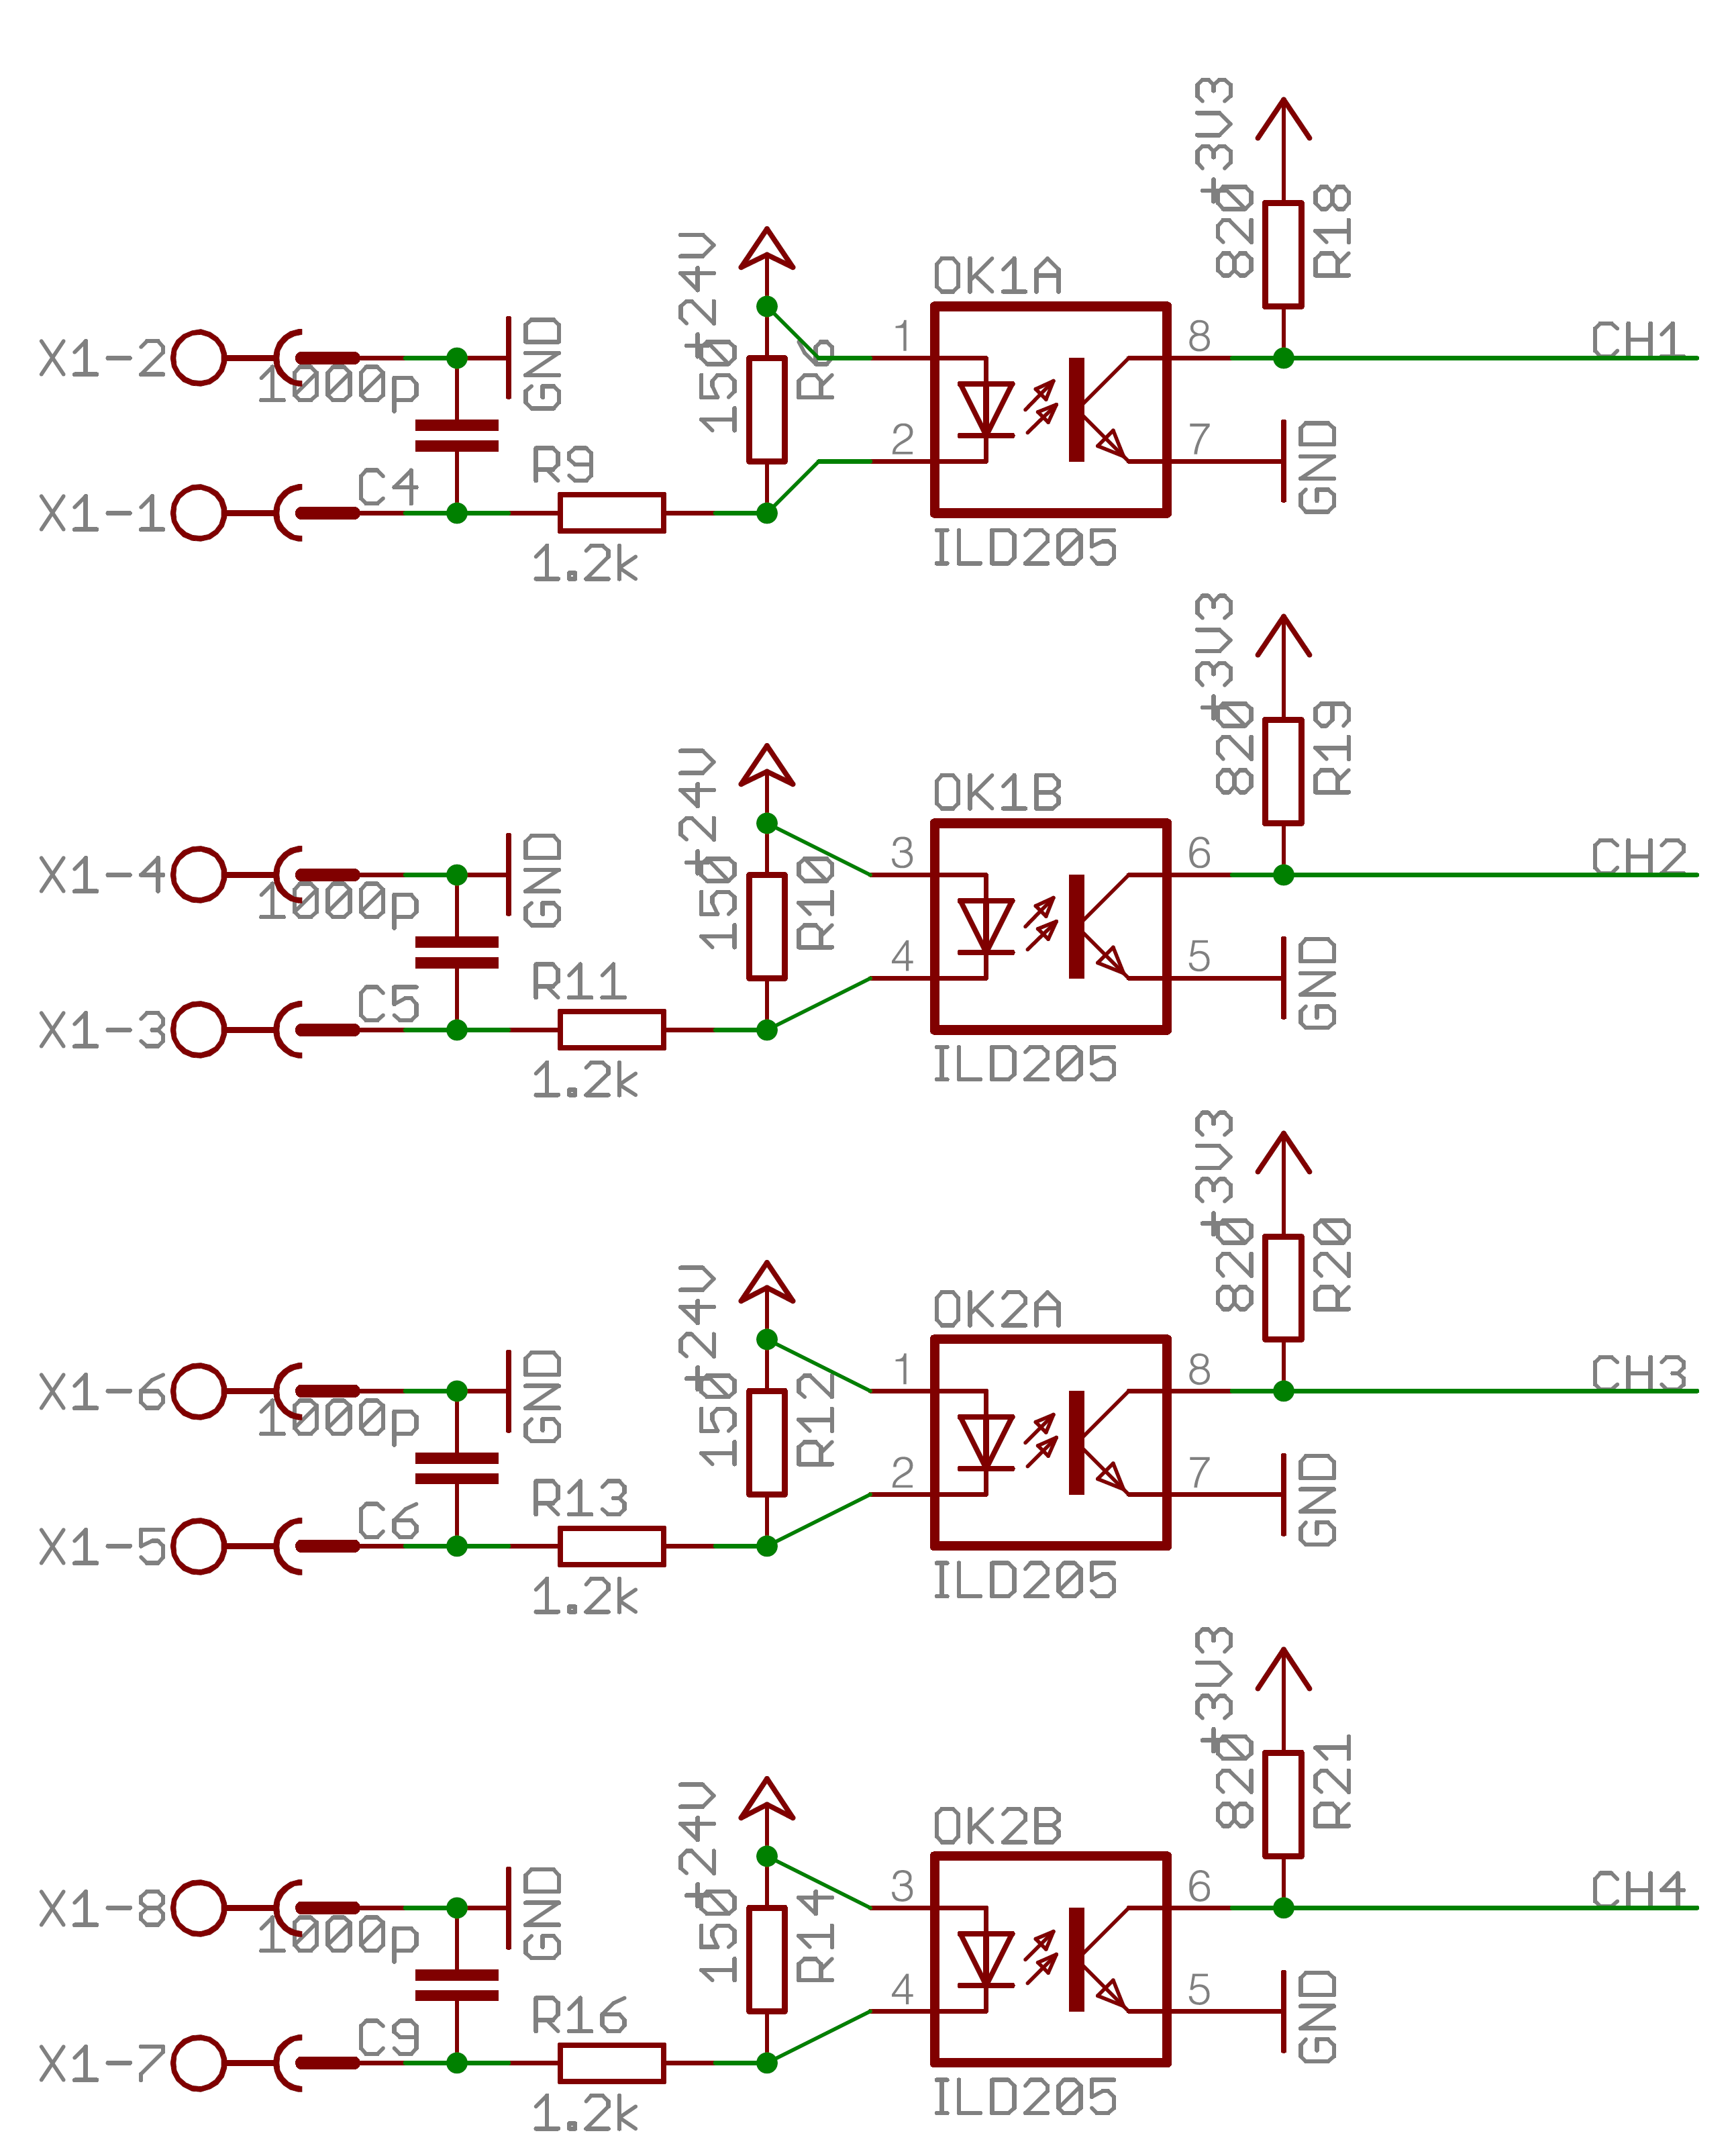
\includegraphics[width=0.60\textwidth]{Bilder/busware_s0.png}
\end{figure}

Zus�tzlich befindet sich eine RJ-10-Schnittstelle sich auf dem SD0. Daneben ist
die Erweiterung mit einem Mikrocontroller, dem Atmega1284p best�ckt. Dieser ist
mit der seriellen Schnittstelle RJ-10-Schnittstelle, den vier S0-Schnittstellen
nach DIN 43864 / EN 62053-31 und der Steckverbindungsleiste verbunden. Zus�tzlich
besitzt die Erweiterung eine Real Time Clock (RTS), die f�r Echtzeitanwendungen
oder hier dem Raspberry Pi zu gute kommen kann [vgl. bsd0 Specs].


\subsection{Real Time Clock (RTC)}
\label{sec:RealTimeClockRTS}

Bei Real Time Clock, kurz RTC bezeichnet, handelt es sich um Echtzeituhren die
Systemzeiten bereitstellen. RTCs stellen also Datum und Uhrzeit bereit [vgl. Bei2011 278].
Beim Real Time Clock des SD0 handelt es sichn um den DS1338U33. Da der Raspberry
Pi ohne einen Internetzugang seine Uhrzeit nicht abgleichen kann, bietet sich die
M�glichkeit an, die Uhrzeit beim RTC des SD0 zu beziehen. Wobei der RTC durch den
Atmega1284p dem Rasperry Pi bereitgestellt wird.

\begin{figure}[htbp]
	\caption{Echtzeituhr des SD0}
	\label{fig:RTC_SD0}
	\centering
		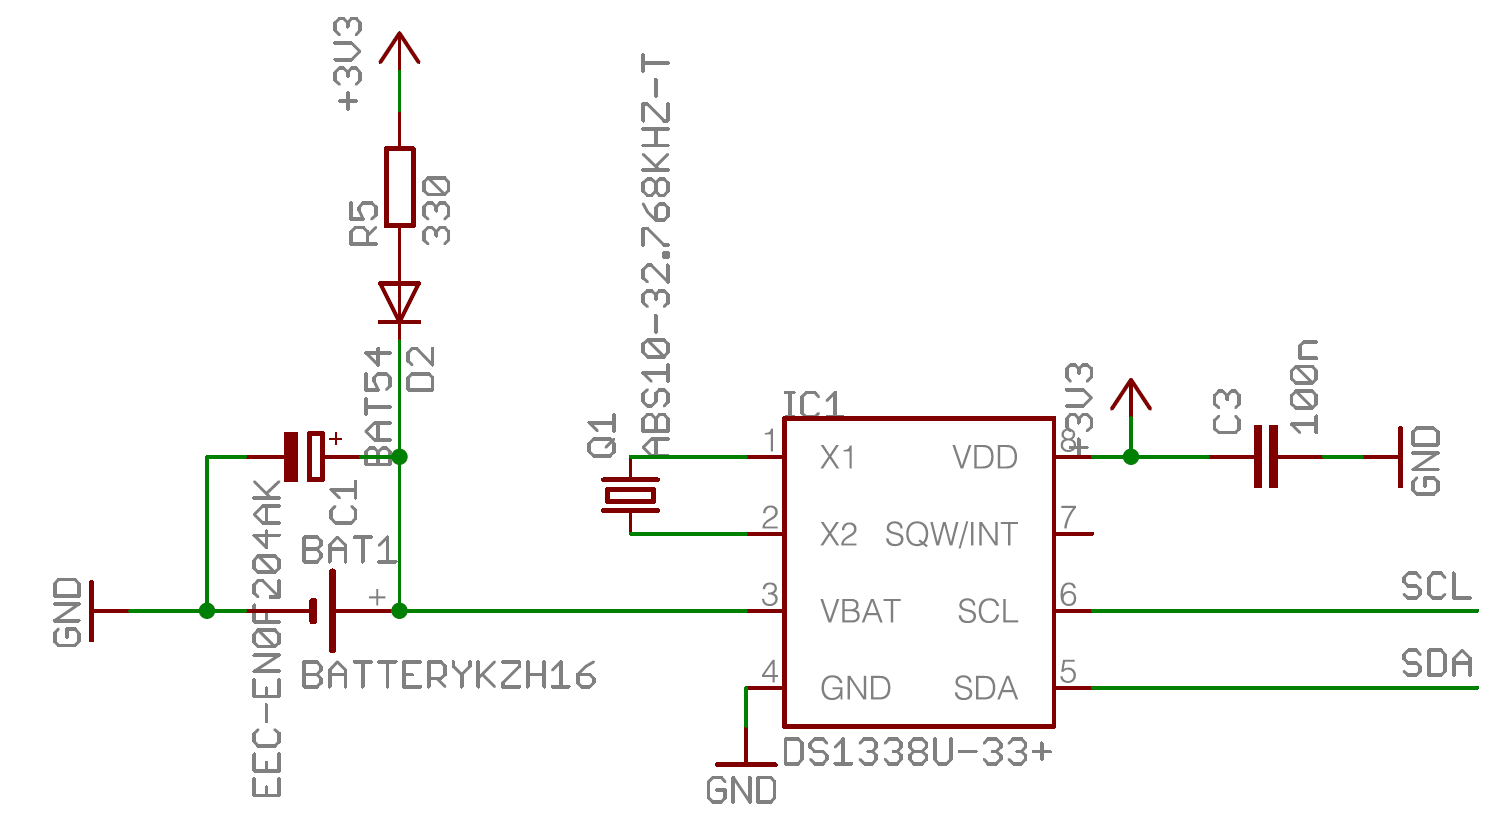
\includegraphics[width=0.70\textwidth]{Bilder/RTC_SD0.png}
\end{figure}

Die Verbindung zur Echtzeituhr wird �ber eine I$^{2}$C Verbindung erstellt. Daf�r
stehen wie in der Abbildung 3.1 dargestellte Leitungen SCL und SDA bereit, welche
jeweils als Takt- und Datenleitung des I$^{2}$C verwendet werden. Es bietet sowohl
die Uhrzeit in den Einheiten Sekunden, Minuten, Stunden als auch den Tag, Monat und
Jahr als Datum an. Die Uhrzeit wird entweder im 12 Stunden oder 24 Stunden Format
bereit-gestellt. Beim 12 Stundenformat indiziert es die AM/PM [vgl. DS1338 S. 1 General Description].
Die Monatsenden werden bei Monaten mit weniger als 31 Tage aut-matisch angepasst.
Es beinhaltet auch die Erkennung von Schaltjahren. Es besitzt einen Stromerkennungssensor.
Es schaltet auf einen 220 mF Kondensator um, wenn es mit zu wenig Strom versorgt wird. [vgl. DS1338 S. 1]


\subsection{Mikrocontroller des SD0}
\label{sec:MikrocontrollerDesSD0}
Neben dem im vorherigen Kapitel beschriebenen RTC ist der SD0 mit einem Mikrocontroller
best�ckt. Bei dem 8-Bit Mikrocontroller handelt es sich um den Atme-ga1284p. Der 8-Bit
Mikrocontroller basiert auf dem AVR. [atm1284 S. 3] �ber das Atmega1284p werden die an
den S0-Schnittstellen empfangenen Daten aufbereitet und an den Ausg�ngen bereitgestellt [bsd0 Specs].


\begin{figure}[htbp]
	\centering
	\caption{Mikrokontroller des SD0}
	\label{fig:SD0_Chanels}
		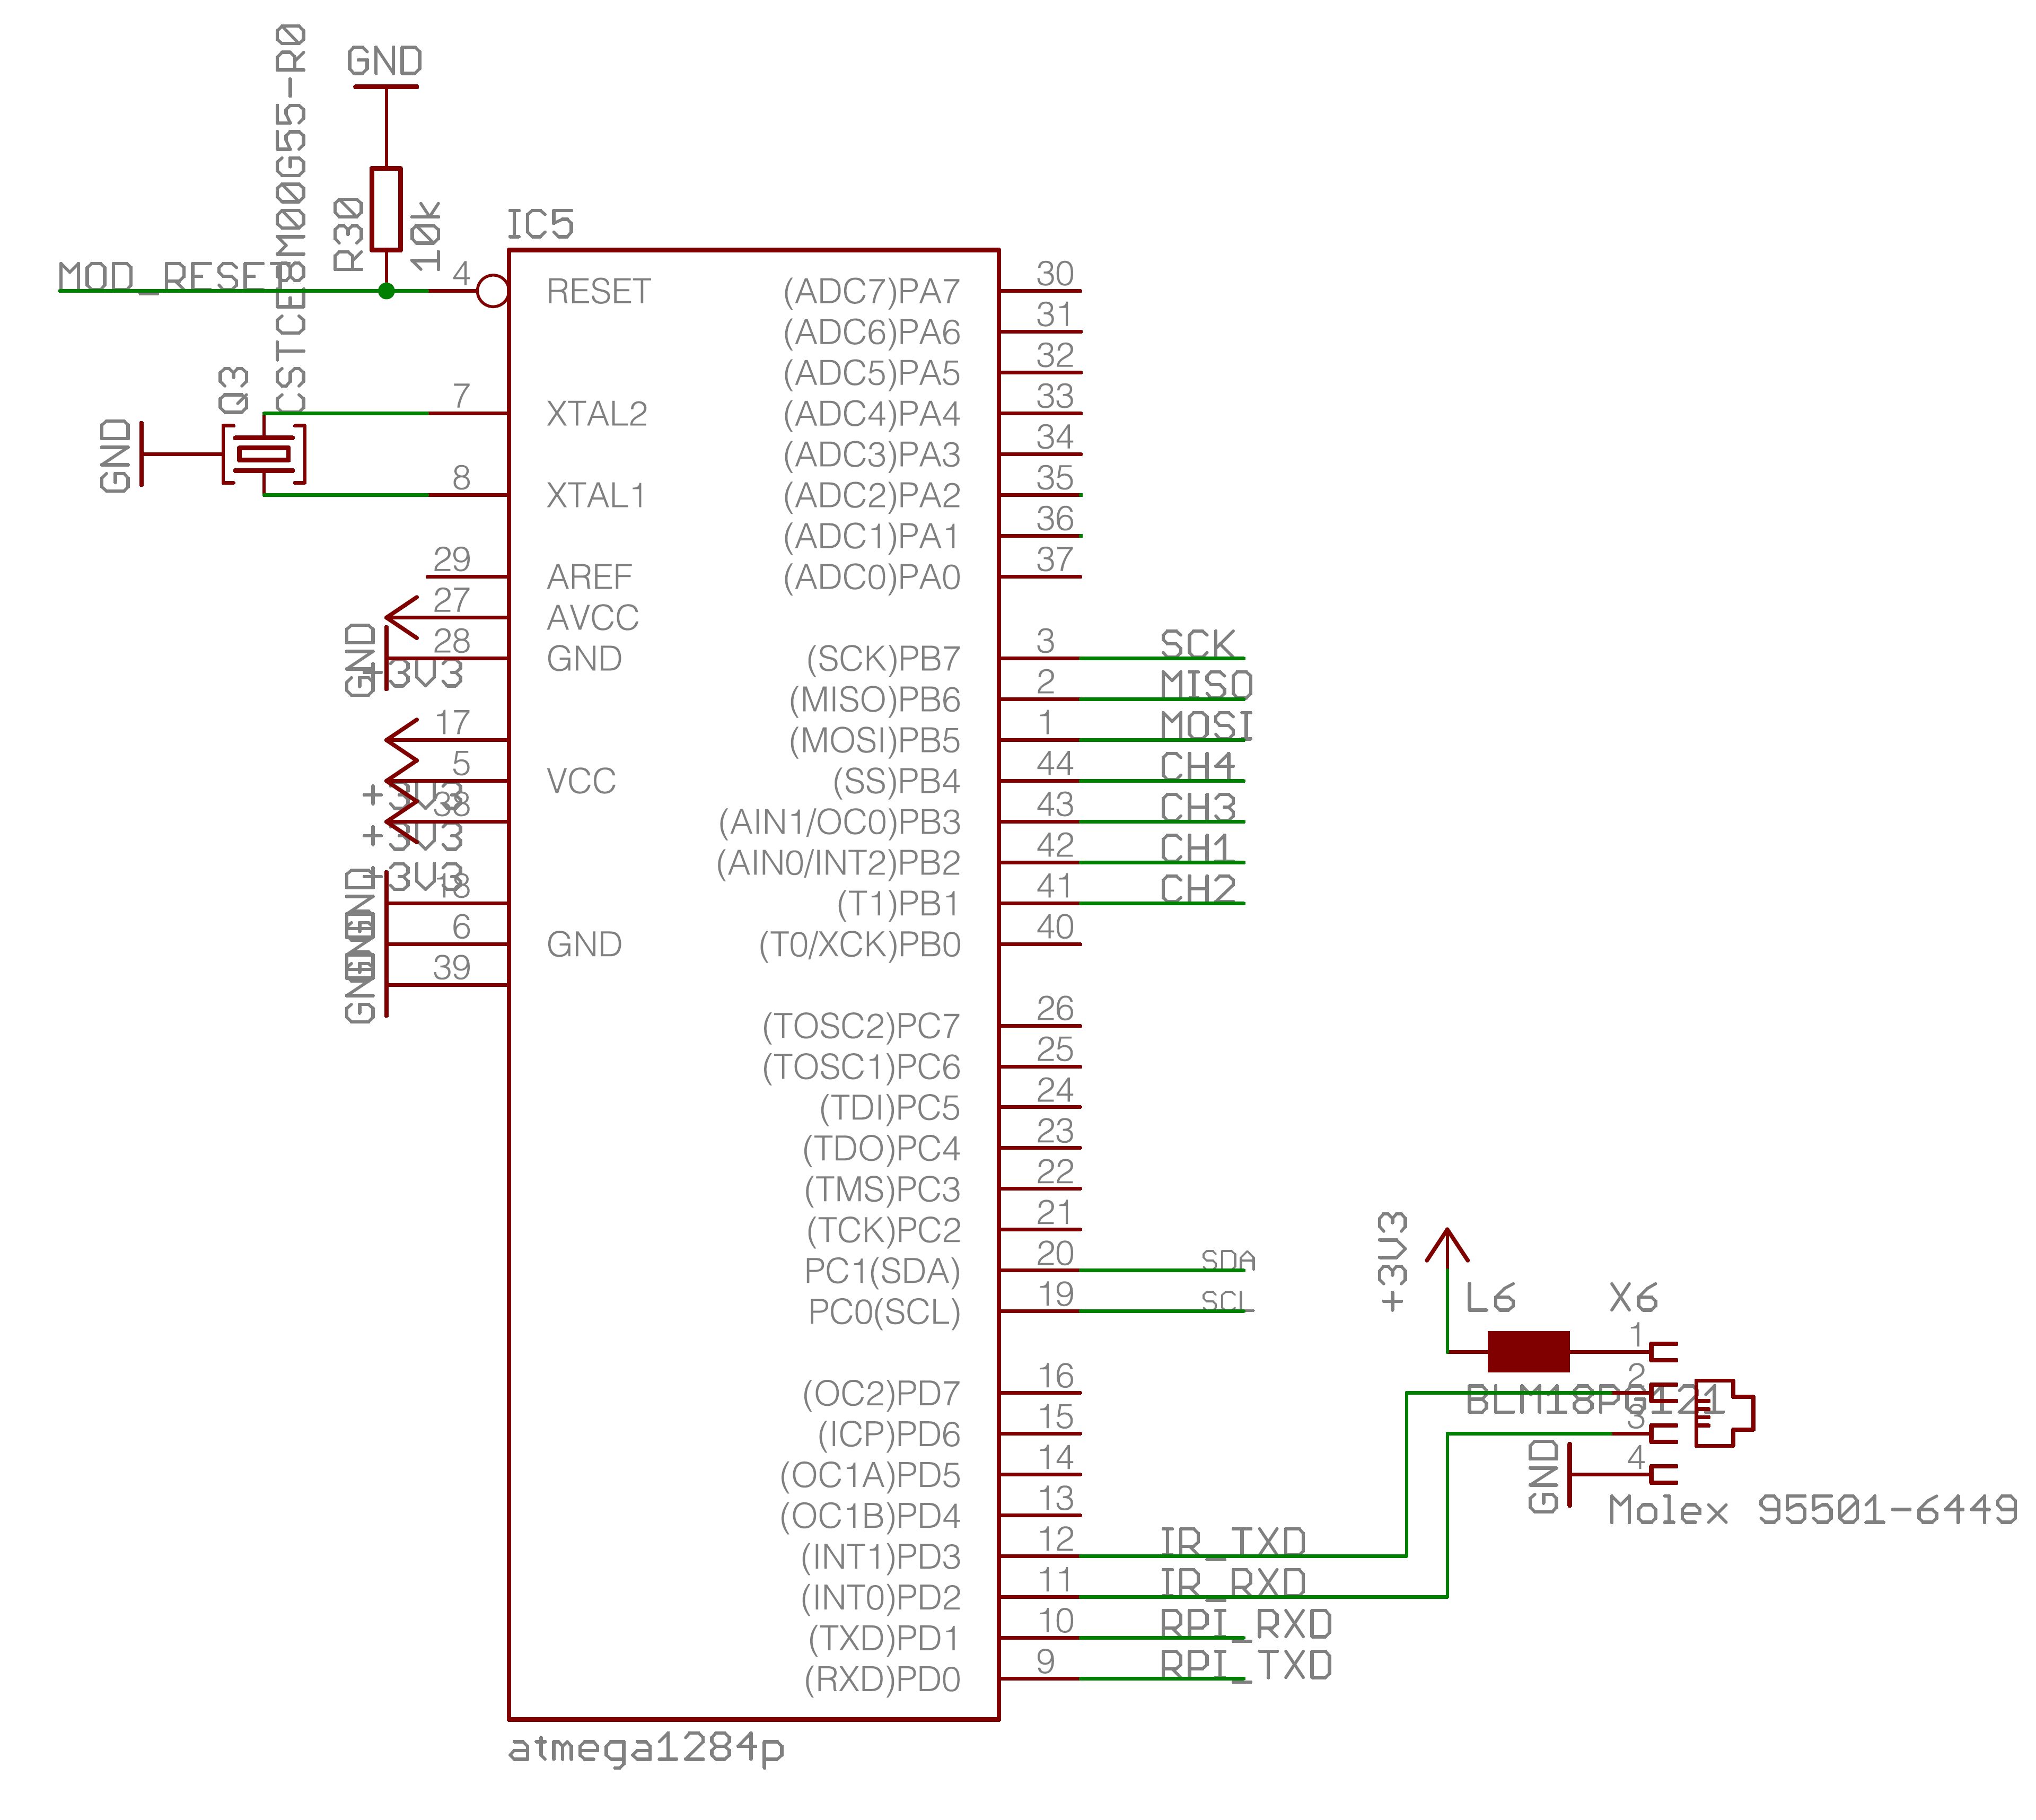
\includegraphics[width=0.50\textwidth]{Bilder/SD0_Chanels.png}
		\center
	\quelle{\cite{sad}}
\end{figure}

Wie der Raspberry besitzt der Atmega 1284p eine GPIO Schnittstelle, beim Amega1284p
besitzt sie jedoch 32 Pins. Durch den Atmega1284p wird auch das RTC bereitgestellt.
Der Mikrocontroller kann �ber zwei USART und eine SPI Schnittstelle kommunizieren. [atm1284 S. 4]
